% \pagebreak[4]
% \hspace*{1cm}
% \pagebreak[4]
% \hspace*{1cm}
% \pagebreak[4]

\chapter{Literature Review}\label{chap:litreview}
\ifpdf
    \graphicspath{{Chapter1/Chapter1Figs/PNG/}{Chapter1/Chapter1Figs/PDF/}{Chapter1/Chapter1Figs/}}
\else
    \graphicspath{{Chapter1/Chapter1Figs/EPS/}{Chapter1/Chapter1Figs/}}
\fi

\section{Issues in Medical Imaging Domain}

This problem has been significantly studied by the research community already (\cite{liu2019comparison}). The major limitation in medical image analysis is the limited size of medical image datasets. Various methods have been formulated over the years to overcome this. Data Augmentation (\cite{perez2017effectiveness}), Active Learning (\cite{hino2020active}) and Transfer Learning (\cite{tan2018survey}) are some of the methods that improved the performance of deep learning models in classification tasks. Data Augmentation generates new data by modifying the existing data slightly which increase the size of dataset. Transfer Learning is the use of pre-trained models for similar tasks which makes learning easier for task-specific models and reduces the training time significantly. Active learning is the method of smartly selecting the algorithm a subset of examples to be labeled next from a set of unlabeled data. 

% Here is an equation\footnote{the notation is explained in the nomenclature section :-)}:
% \begin{eqnarray}
% CIF: \hspace*{5mm}F_0^j(a) &=& \frac{1}{2\pi \iota} \oint_{\gamma} \frac{F_0^j(z)}{z - a} dz
% \end{eqnarray}
% \nomenclature[zcif]{$CIF$}{Cauchy's Integral Formula}                                % first letter Z is for Acronyms 
% \nomenclature[aF]{$F$}{complex function}                                                   % first letter A is for Roman symbols
% \nomenclature[gp]{$\pi$}{ $\simeq 3.14\ldots$}                                             % first letter G is for Greek Symbols
% \nomenclature[gi]{$\iota$}{unit imaginary number $\sqrt{-1}$}                      % first letter G is for Greek Symbols
% \nomenclature[gg]{$\gamma$}{a simply closed curve on a complex plane}  % first letter G is for Greek Symbols
% \nomenclature[xi]{$\oint_\gamma$}{integration around a curve $\gamma$} % first letter X is for Other Symbols
% \nomenclature[rj]{$j$}{superscript index}                                                       % first letter R is for superscripts
% \nomenclature[s0]{$0$}{subscript index}                                                        % first letter S is for subscripts

\section{Inductive Bias}
The commonality among the above methods is that they extract relevant features which can be achieved by modelling and incorporating appropriate inductive biases. Inductive biases are defined as a set of assumptions used by a learner to predict outputs. Inducing biases can avoid learning of invalid correlations which leads to shortcut learning. When a model learns in a shortcut manner, then it will perform poorly in real-world scenarios even when it can perform well in benchmark datasets. A robust and an effective inductive bias eliminates shortcut learning by guiding the model to learn correct features of the model. This can be done in various ways by considering model architecture, loss functions, data selection, and model optimization.

\section{Saliency Maps}

A lot of research has been done to generate interpretable explanations for the trained models. Local Interpretable Model Agnostic Explanations (LIME) (\cite{ribeiro2016why}) was one of the first papers to delve into the field of model explainability. It achieved breakthrough in this domain by explaining the predictions of a machine learning model with the help of a locally built model which can be interpreted. Saliency map is one of the most frequently used explanation methods to interpret the predictions of an image classification model. The saliency map is generated by backpropagating from the output layer to the input layer and taking the gradients into account. It highlights the important features of the images that were relevant for classification.

Researchers have come up with various methods to generate different variants of saliency maps over the years. Grad-CAM (\cite{selvaraju2017grad}) uses the gradients flowing from the prediction layer to the last convolutional layer to generate a coarse localization map which highlights the important features in the image that were used for prediction. DeepTaylor (\cite{montavon2017explaining}) is an innovative method based on Taylor expansions which decomposes the output of a deep neural network in terms of input variables. LRP \cite{binder2016layer} is a method which decomposes the prediction of a deep neural network computed over an image to relevance scores for the single input dimensions of the image. The above methods are some of the commonly used methods to visualize the predictions of a deep neural network.

\section{Model Calibration}

Calibration evaluation of neural networks in classification tasks has been a research topic for over a decade. There are various ways to calibrate a model such as post-hoc rescaling of predictions (\cite{guo2017calibration}), averaging multiple predictions (\cite{lakshminarayanan2017simple}, \cite{wen2020batchensemble}), and data augmentation (\cite{thulasidasan2019mixup}, \cite{wen2020combining}). However, we focus on post processing of predictions to make medical image classification systems more reliable.

\cite{niculescu2005predicting} used classical reliability diagrams (\cite{murphy1977reliability}) to investigate calibration of shallow neural networks in a binary
classification setting and concluded that these networks are
well-calibrated. \cite{guo2017calibration} showed empirically that  modern neural networks are no longer well-calibrated, despite the improvement of accuracy of neural networks, and ignited a strand of research (\cite{kumar2018trainable}, \cite{zhang2018noisy}, \cite{kendall2017uncertainties})
proposing methods for obtaining calibrated classifiers. In
all these works, calibration of the classifier is judged based
on classical reliability diagrams and the so-called expected
calibration error (ECE) (\cite{guo2017calibration}) whose real-valued
estimate is calculated from a reliability diagram and its associated confidence histogram.


% Now I would like to cite the following: \cite{latex} and \cite{texbook}
% and \cite{Rud73}.

% I would also like to include a picture ...

% \begin{figure}[!htbp]
%   \begin{center}
%     \leavevmode
%     \ifpdf
%       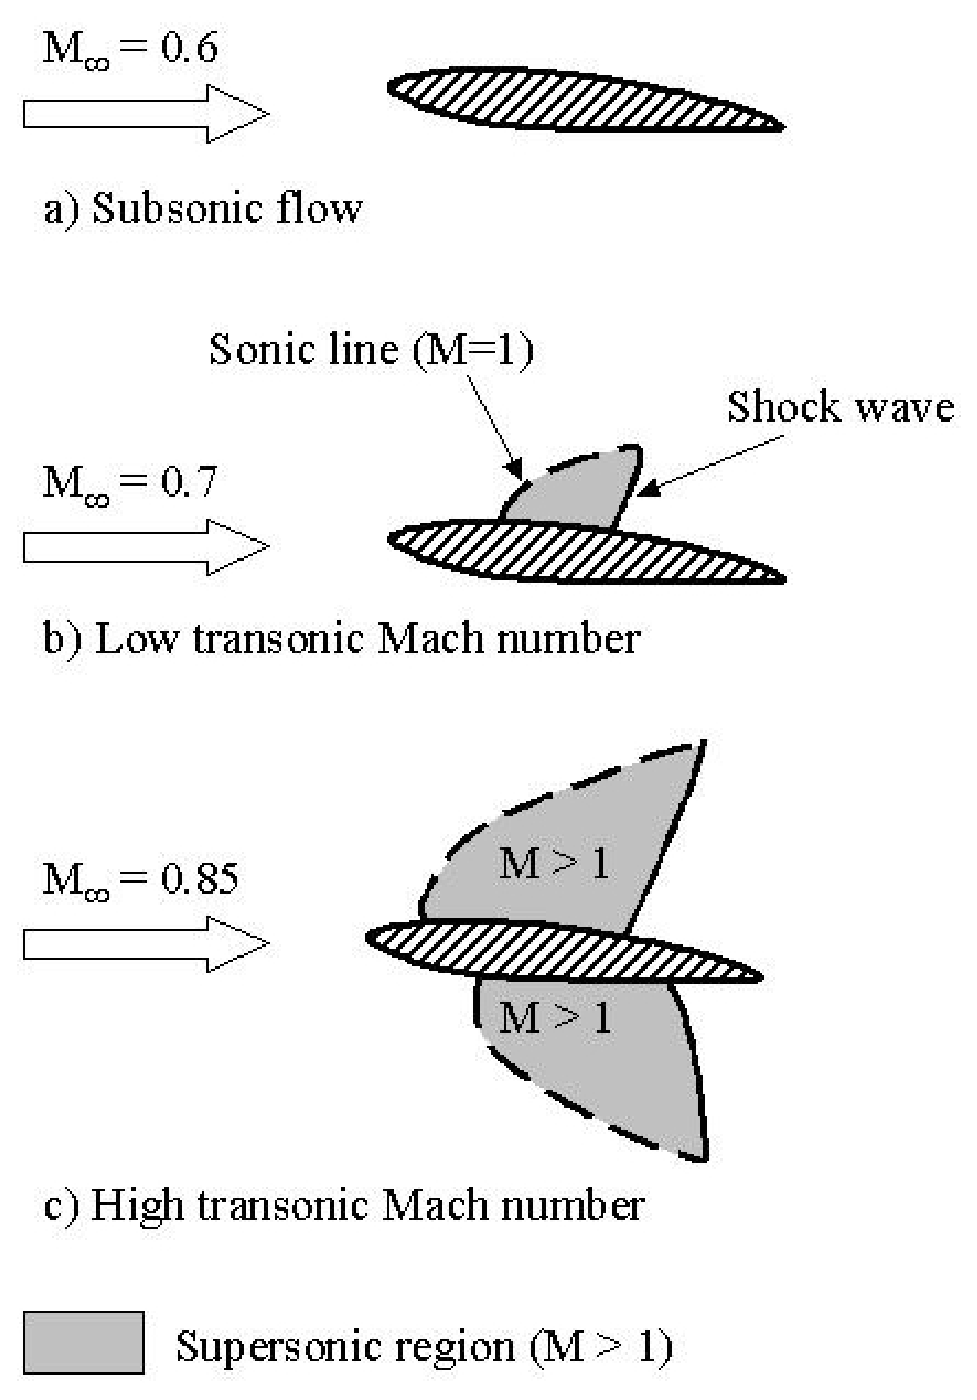
\includegraphics[height=6in]{aflow}
%     \else
%       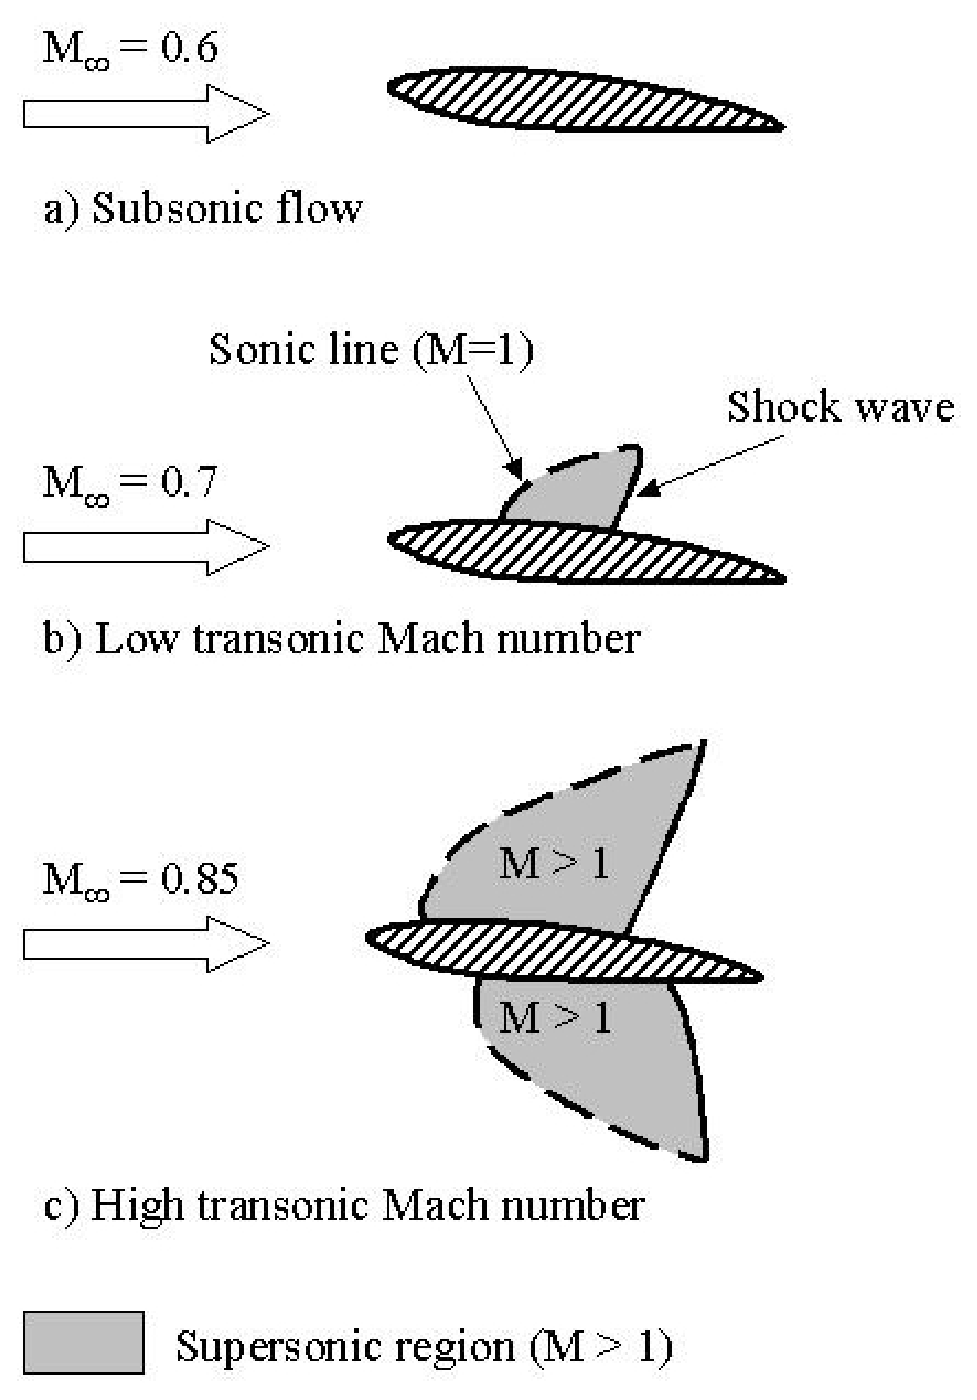
\includegraphics[bb = 92 86 545 742, height=6in]{aflow}
%     \fi
%     \caption{Airfoil Picture}
%     \label{FigAir}
%   \end{center}
% \end{figure}

% above code has been macro-fied in Classes/MacroFile.tex file
%\InsertFig{\IncludeGraphicsH{aflow}{6in}{92 86 545 742}}{Airfoil Picture}{FigAir}

% So as we have now labelled it we can reference it, like so (\ref{FigAir}) and it
% is on Page \pageref{FigAir}. And as we can see, it is a very nice picture and we
% can talk about it all we want and when we are tired we can move on to the next
% chapter ...

% I would also like to add an extra bookmark in acroread like so ...
% \ifpdf
%   \pdfbookmark[2]{bookmark text is here}{And this is what I want bookmarked}
% \fi
% ------------------------------------------------------------------------


%%% Local Variables: 
%%% mode: latex
%%% TeX-master: "../thesis"
%%% End: 
